\begin{frame}[allowframebreaks]{}
    \LARGE Normalizing Flow Models: \\[1.5ex] \textbf{Change of Variables Theorem}
\end{frame}

\begin{frame}[allowframebreaks]{Change of Variables Theorem}
The change of variables formula describe how to evaluate densities of a random variable that is a deterministic transformation from another variable.
\begin{figure}
    \centering
        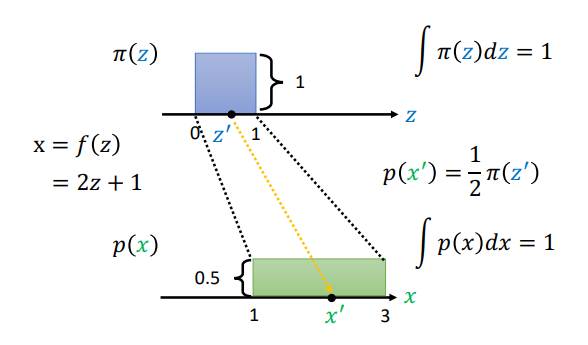
\includegraphics[height=0.6\textheight, width=\textwidth, keepaspectratio]{images/norm-flow/change_var.png}
        \caption*{Transformation of a 1-D random variable to another random variable. Note that the areas of the blue and green rectangles are equal.}
\end{figure}

\framebreak
\begin{figure}
    \centering
    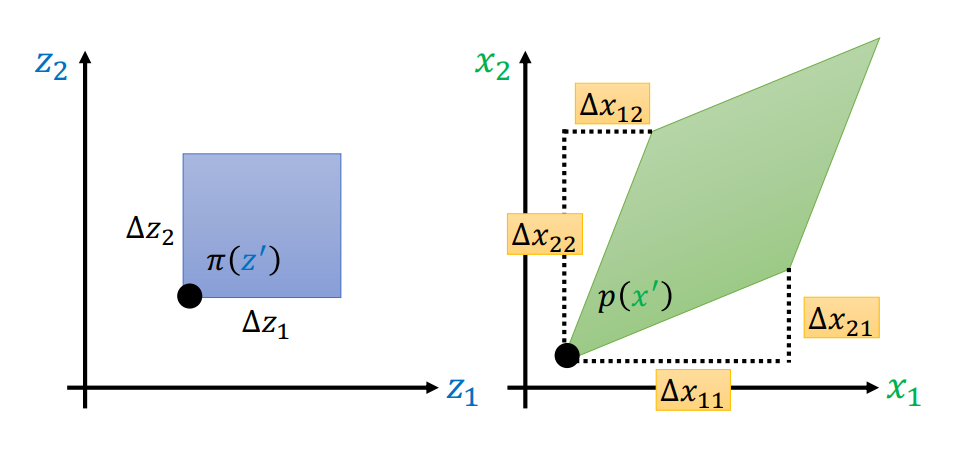
\includegraphics[height=0.7\textheight, width=\textwidth, keepaspectratio]{images/norm-flow/change_var_2.png}
    \caption*{Transformation of a 2-D random variable to another random variable. Note that the areas of the blue and green rectangles are equal.}
\end{figure}

\framebreak

\textbf{Theorem}: Let $Z$ and $X$ be random variables related by a mapping $f:\mathbb{R}^n \rightarrow \mathbb{R}^n$ such that $X = f(Z)$ and $Z = f^{-1}(X)$. Then,
\[
p_X(x) = p_Z(f^{-1}(x)) \left| \det \left( \frac{\partial f^{-1}(x)}{\partial x} \right) \right|
\]
Some important points to note:
\begin{itemize}
    \item $x$ and $z$ must be continuous random variables of the same dimension.
    \item $\frac{\partial f^{-1}(x)}{\partial x}$ is the $n \times n$ \textbf{Jacobian matrix}, where the entry at position $(i, j)$ is $\frac{\partial [f^{-1}(x)]_i}{\partial x_j}$.
    \item For any invertible matrix $A$, $\det(A^{-1}) = [\det(A)]^{-1}$. Therefore, for $z = f^{-1}(x)$,
    \[
    p_X(x) = p_Z(z) \left| \det \left( \frac{\partial f(z)}{\partial z} \right) \right|^{-1}
    \]
\end{itemize}

\framebreak

\large We need:
\begin{itemize}
    \item \textbf{Invertibility of $f$}: The function $f$ must be invertible so that for every $x$ there exists a unique $z = f^{-1}(x)$.
    \item \textbf{Jacobian of $f$}: The Jacobian matrix $\frac{\partial f(z)}{\partial z}$ must be computable and its determinant non-zero almost everywhere to ensure the change of variables formula is valid.
\end{itemize}

\end{frame}